\documentclass[11pt,a4paper]{article}
\usepackage[T1]{fontenc}
\usepackage[utf8]{inputenc}
\usepackage[provide=*,french]{babel}
\usepackage{lmodern}
\usepackage{geometry,graphicx,xcolor,tikz,booktabs,array,float}
\usepackage{amsmath}
\usepackage[hidelinks]{hyperref}
\usetikzlibrary{calc}
\geometry{left=2.1cm,right=2.1cm,top=1.9cm,bottom=2cm}
\definecolor{inseagreen}{RGB}{1,135,84}
\definecolor{subjectbadge}{RGB}{121,182,149}
\definecolor{subjectbg}{RGB}{196,220,206}
\definecolor{subjectborder}{RGB}{121,182,149}
\graphicspath{{figures/}{figures/logos/}{../figures/}}
\hypersetup{pdftitle={Prédiction des besoins énergétiques des bâtiments},
 pdfauthor={ELKIHEL ELMEHDI, EL ASSRI L'HOUCINE, SAID CHARAF}}
\begin{document}
% Adaptation au mini-projet 03. Le modèle transmis concernait un autre stage.
\begin{titlepage}
\thispagestyle{empty}
\begin{tikzpicture}[remember picture,overlay]
  \foreach \i in {0,...,7}{
    \draw[inseagreen,line width=.7pt]
      ([xshift={6.4cm+\i*.45cm}]current page.north west)
      .. controls ([xshift={6cm+\i*.45cm},yshift=-4cm]current page.north west)
      and ([xshift=1cm,yshift=-5cm]current page.north west)
      .. ([yshift={-8cm-\i*.45cm}]current page.north west);
  }
  \fill[inseagreen!80]
    ([xshift=-6cm]current page.south east)
    .. controls ([xshift=-5.8cm,yshift=3cm]current page.south east)
    and ([xshift=-1cm,yshift=5cm]current page.south east)
    .. ([yshift=8cm]current page.south east)
    -- (current page.south east) -- cycle;
\end{tikzpicture}
\centering
\vspace*{.2cm}
\begin{minipage}[c]{.54\textwidth}
\raggedright\small\bfseries ROYAUME DU MAROC\\[.12cm]
HAUT-COMMISSARIAT AU PLAN\\[.12cm]
INSTITUT NATIONAL DE STATISTIQUE\\
ET D'ÉCONOMIE APPLIQUÉE
\end{minipage}\hfill
\begin{minipage}[c]{.29\textwidth}
\raggedleft
\includegraphics[width=3.2cm]{figures/logos/INSEA_logo.png}
\end{minipage}
\vspace{2.6cm}

{\Large\bfseries Rapport de mini-projet de Machine Learning\par}
\vspace{.25cm}
{\large Mini-projet 03\par}
\vspace{1.2cm}
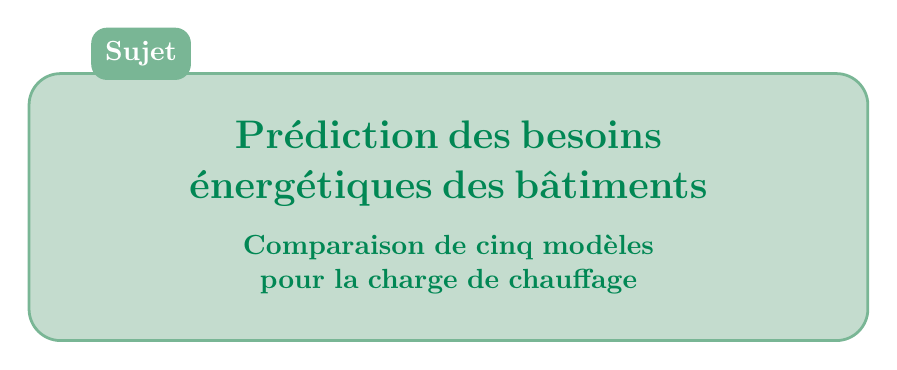
\begin{tikzpicture}
\node[draw=subjectborder,fill=subjectbg,rounded corners=4mm,
  line width=1pt,inner sep=17pt,text width=.78\textwidth,align=center] (box)
  {\Large\bfseries\color{inseagreen} Prédiction des besoins énergétiques des bâtiments\\[.3cm]
   \normalsize Comparaison de cinq modèles pour la charge de chauffage};
\node[anchor=south west,xshift=.8cm,yshift=-3pt,
  fill=subjectbadge,rounded corners=2mm,inner sep=5pt,text=white]
  at (box.north west) {\textbf{Sujet}};
\end{tikzpicture}
\vspace{1.3cm}

{\bfseries Réalisé par\par}\vspace{.25cm}
ELKIHEL ELMEHDI\\[.13cm]
EL ASSRI L'HOUCINE\\[.13cm]
SAID CHARAF

\vfill
{\large\bfseries Année universitaire 2026--2027\par}
\vspace{.2cm}
\end{titlepage}

\setcounter{page}{1}
\section{Contexte et données}
La charge de chauffage d'un bâtiment dépend de sa géométrie et de ses vitrages. Ce mini-projet compare cinq méthodes de régression afin de prédire cette charge à partir du jeu public \emph{Energy Efficiency} de l'UCI. L'objectif est double : comparer les approches linéaires et non linéaires et examiner les cas où le modèle commet les plus fortes erreurs. Il s'agit d'une étude de configurations \emph{simulées}, et non d'une validation sur des bâtiments réels.

Le fichier contient 768 lignes sans valeur manquante. Les huit entrées sont $X_1$ (compacité relative), $X_2$ (surface), $X_3$ (surface des murs), $X_4$ (surface du toit), $X_5$ (hauteur), $X_6$ (orientation), $X_7$ (surface vitrée) et $X_8$ (distribution des vitrages). La cible unique est $Y_1$, charge de chauffage. La seconde sortie $Y_2$, charge de refroidissement, est exclue des entrées et des modèles. L'orientation et la distribution des vitrages sont encodées comme des catégories, pour ne pas imposer un ordre numérique artificiel.

\begin{figure}[H]\centering
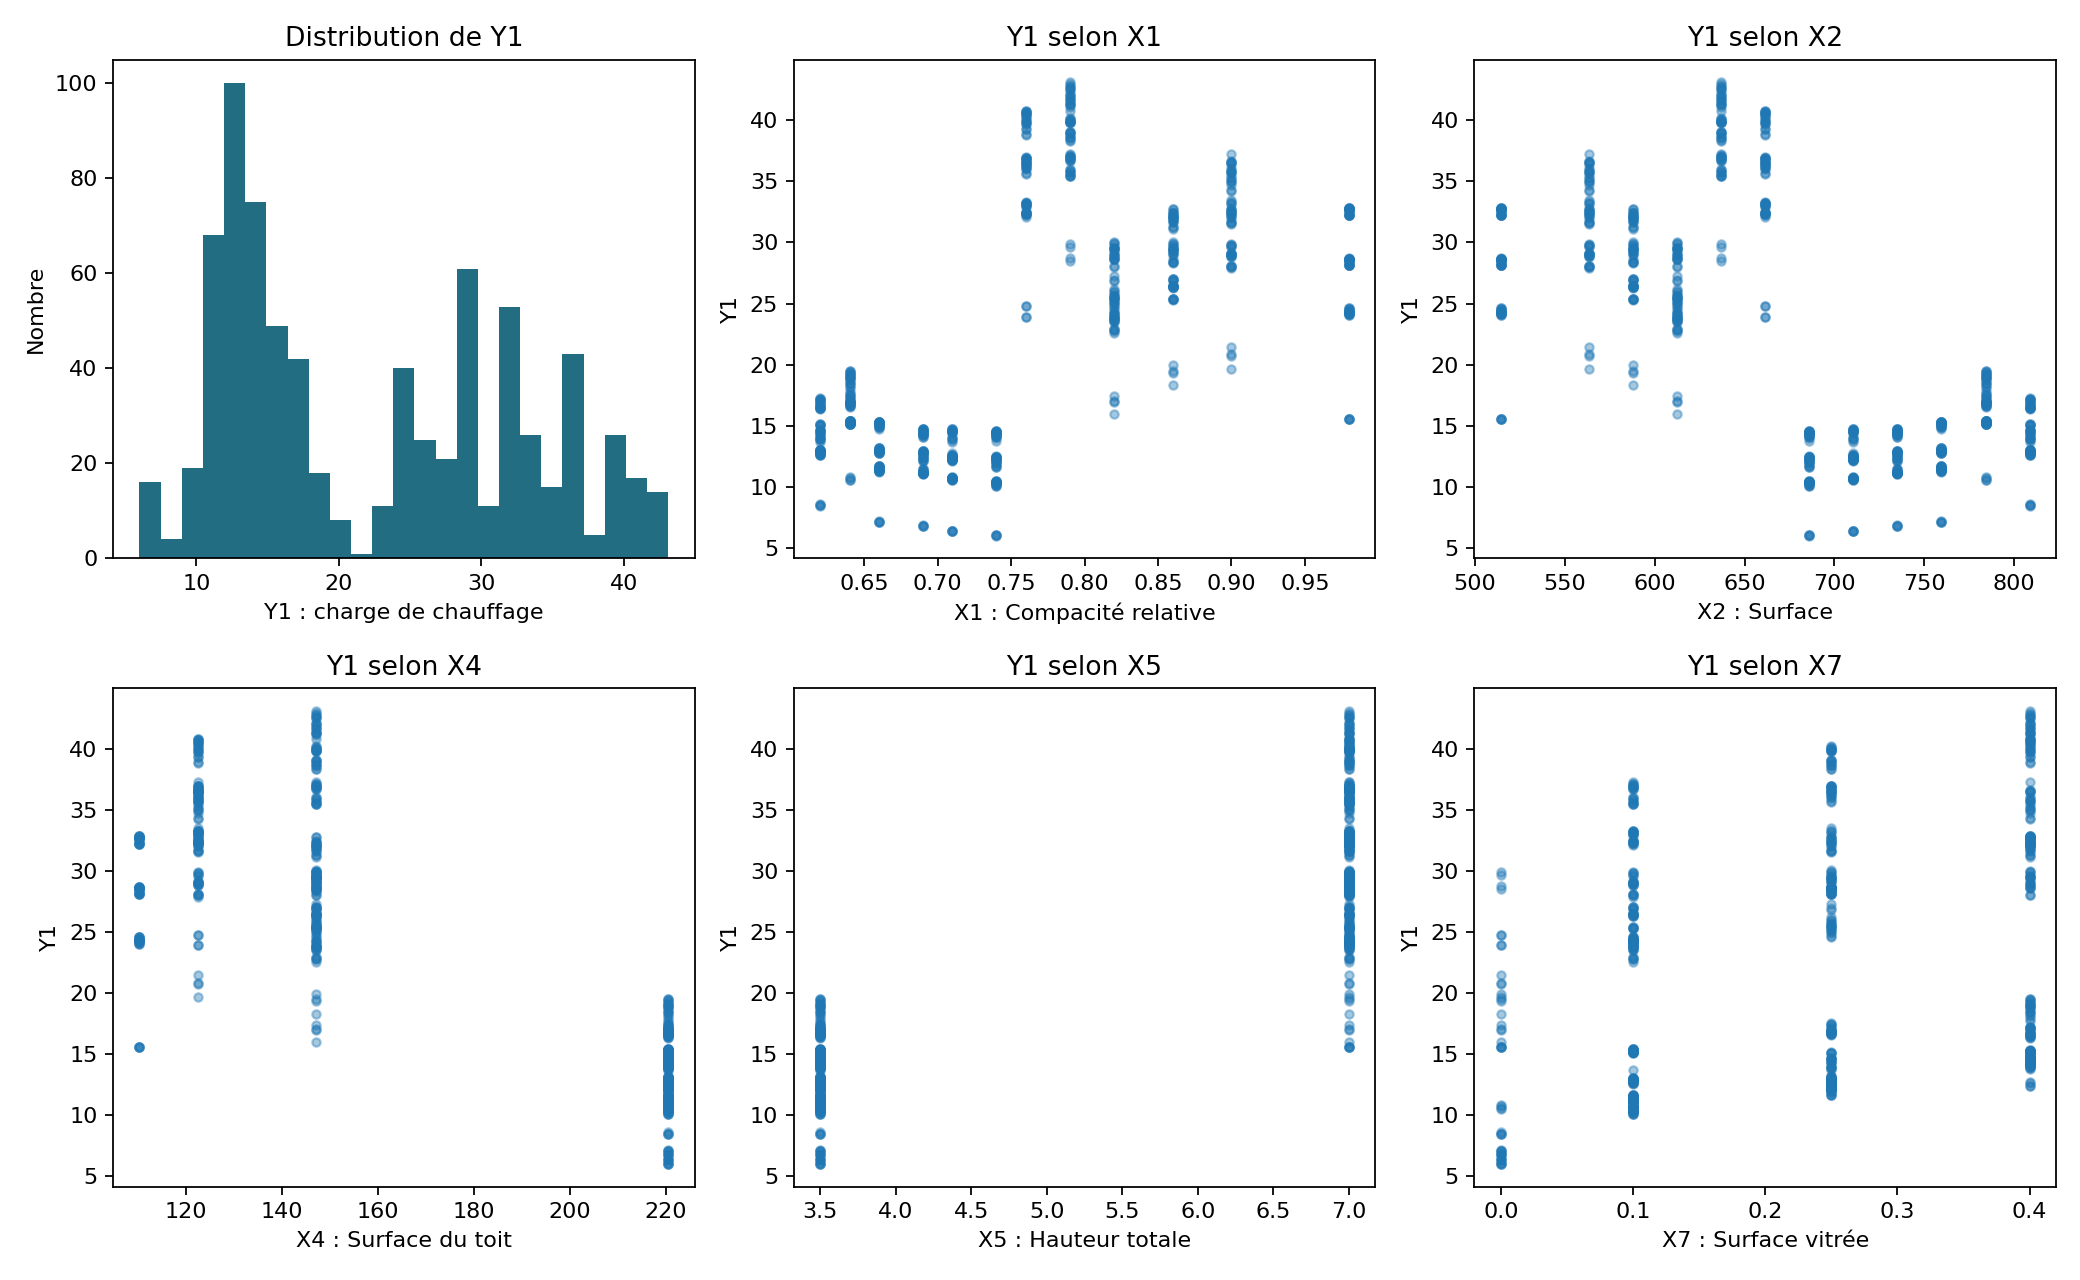
\includegraphics[width=.94\linewidth]{01_exploration.png}
\caption{Distribution de $Y_1$ et relations descriptives avec cinq caractéristiques. Les observations sont simulées.}
\end{figure}
\noindent La distribution de $Y_1$ est étalée et les relations avec les caractéristiques ne semblent pas toutes linéaires. Les graphiques sont descriptifs ; ils ne suffisent pas à établir un effet causal d'une variable sur la consommation.
\clearpage
\section{Protocole expérimental}
Nous utilisons une séparation aléatoire fixée par \texttt{random\_state=42} : 614 observations (80\,\%) pour l'entraînement et 154 (20\,\%) pour le test. Sur l'entraînement uniquement, une validation croisée à cinq plis, mélangés avec la même graine, compare les réglages selon le RMSE moyen. Le test est réservé au calcul final des métriques.

La régression linéaire constitue la référence sans hyperparamètre réglé. Ridge ajoute une pénalisation $L_2$ dont le coefficient $\alpha$ est choisi par validation. KNN compare plusieurs nombres de voisins, distances et pondérations. L'arbre de décision compare profondeur et taille minimale des feuilles. Random Forest compare le nombre d'arbres, leur profondeur et la taille minimale des feuilles. Les grilles exactes et les paramètres retenus sont conservés dans le code et dans \texttt{results/parameters.json}.

Les six variables quantitatives sont standardisées pour les modèles sensibles à l'échelle (linéaire, Ridge et KNN). La standardisation n'est pas nécessaire pour les modèles arborescents. Chaque transformation est dans le pipeline : pendant un pli, elle est ajustée sur la seule sous-partie d'apprentissage. Cela évite de transmettre à l'entraînement des informations provenant de la validation ou du test.

Pour une vraie valeur $y_i$ et sa prédiction $\hat y_i$, nous calculons :
\[
\mathrm{MAE}=\frac1n\sum_i|y_i-\hat y_i|,\qquad
\mathrm{MSE}=\frac1n\sum_i(y_i-\hat y_i)^2,\qquad
\mathrm{RMSE}=\sqrt{\mathrm{MSE}}.
\]
Le coefficient $R^2=1-\sum_i(y_i-\hat y_i)^2/\sum_i(y_i-\bar y)^2$ compare l'erreur du modèle à celle d'une prédiction constante égale à la moyenne du test. Les trois mesures d'erreur sont meilleures lorsqu'elles diminuent ; $R^2$ est meilleur lorsqu'il se rapproche de 1.

\section{Résultats sur les 154 observations de test}
\begin{table}[H]\centering\small
\begin{tabular}{lrrrrr}\toprule
Modèle & RMSE CV & MAE & MSE & RMSE & $R^2$\\\midrule
Régression linéaire & 2,828 & 2,059 & 8,250 & 2,872 & 0,921\\
Ridge & 2,828 & 2,061 & 8,257 & 2,874 & 0,921\\
KNN & 1,559 & 1,118 & 2,793 & 1,671 & 0,973\\
Arbre de décision & 0,579 & 0,353 & 0,282 & \textbf{0,531} & \textbf{0,997}\\
Random Forest & \textbf{0,535} & 0,371 & 0,287 & 0,536 & 0,997\\\bottomrule
\end{tabular}
\caption{Comparaison des cinq modèles. RMSE CV : moyenne de validation croisée sur l'entraînement ; autres colonnes : test. Valeurs arrondies.}
\end{table}
\begin{figure}[H]\centering
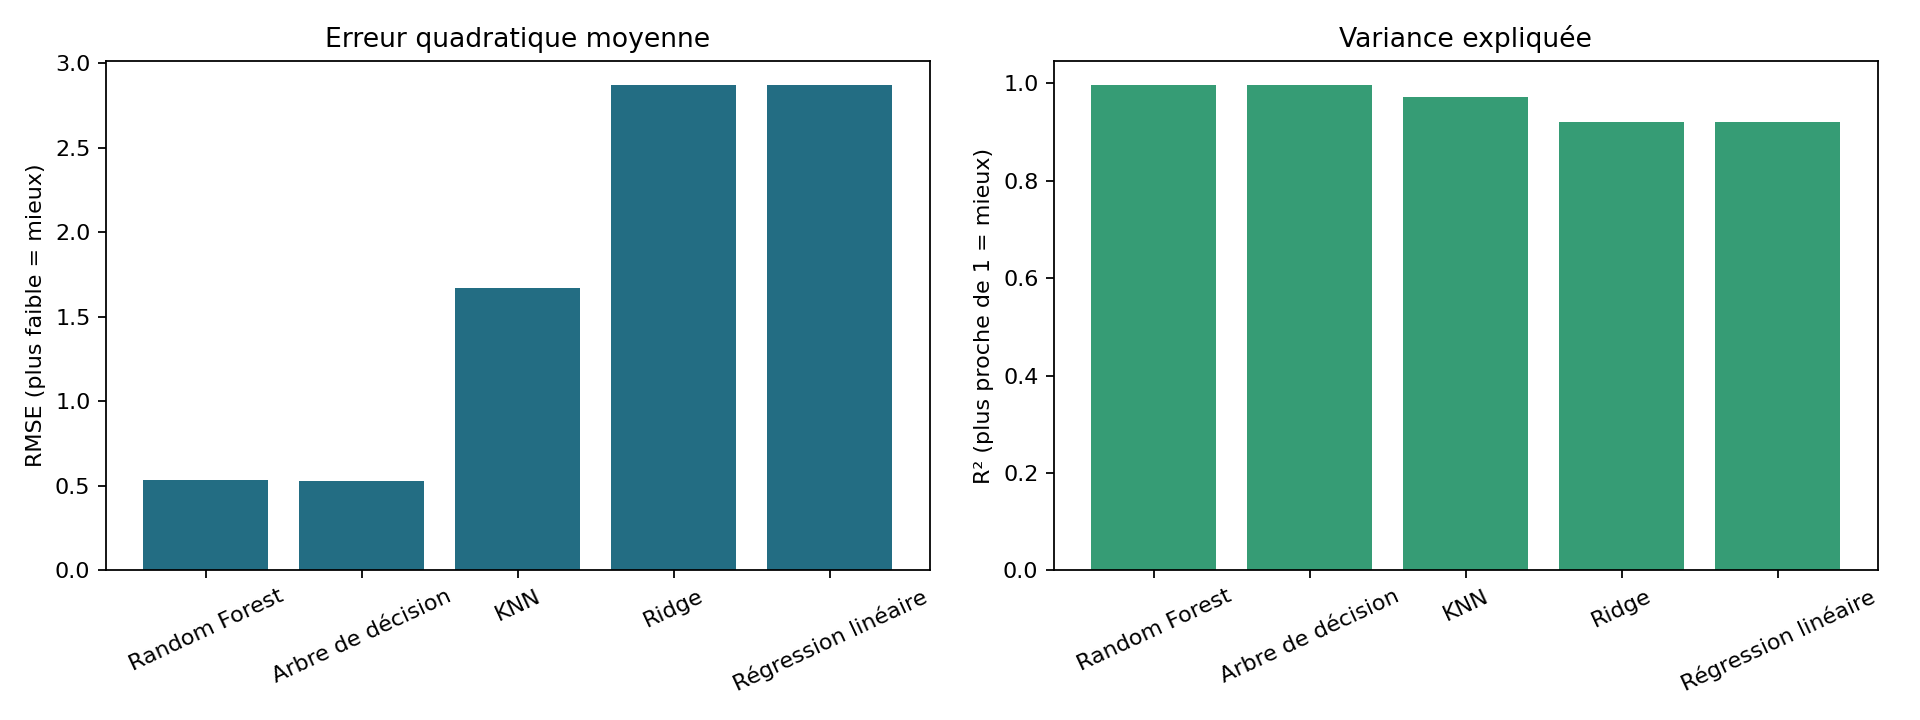
\includegraphics[width=.72\linewidth]{02_comparaison.png}
\caption{Comparaison visuelle du RMSE et du $R^2$ sur le test.}
\end{figure}
Random Forest présente le plus faible RMSE de validation croisée et constitue donc le modèle sélectionné avant l'examen du test. L'arbre obtient un RMSE de test légèrement plus faible (0,531 contre 0,536) sur cette partition précise. Cette faible différence ne démontre pas une supériorité générale.
\clearpage
\section{Prédictions, erreurs et discussion}
\begin{figure}[H]\centering
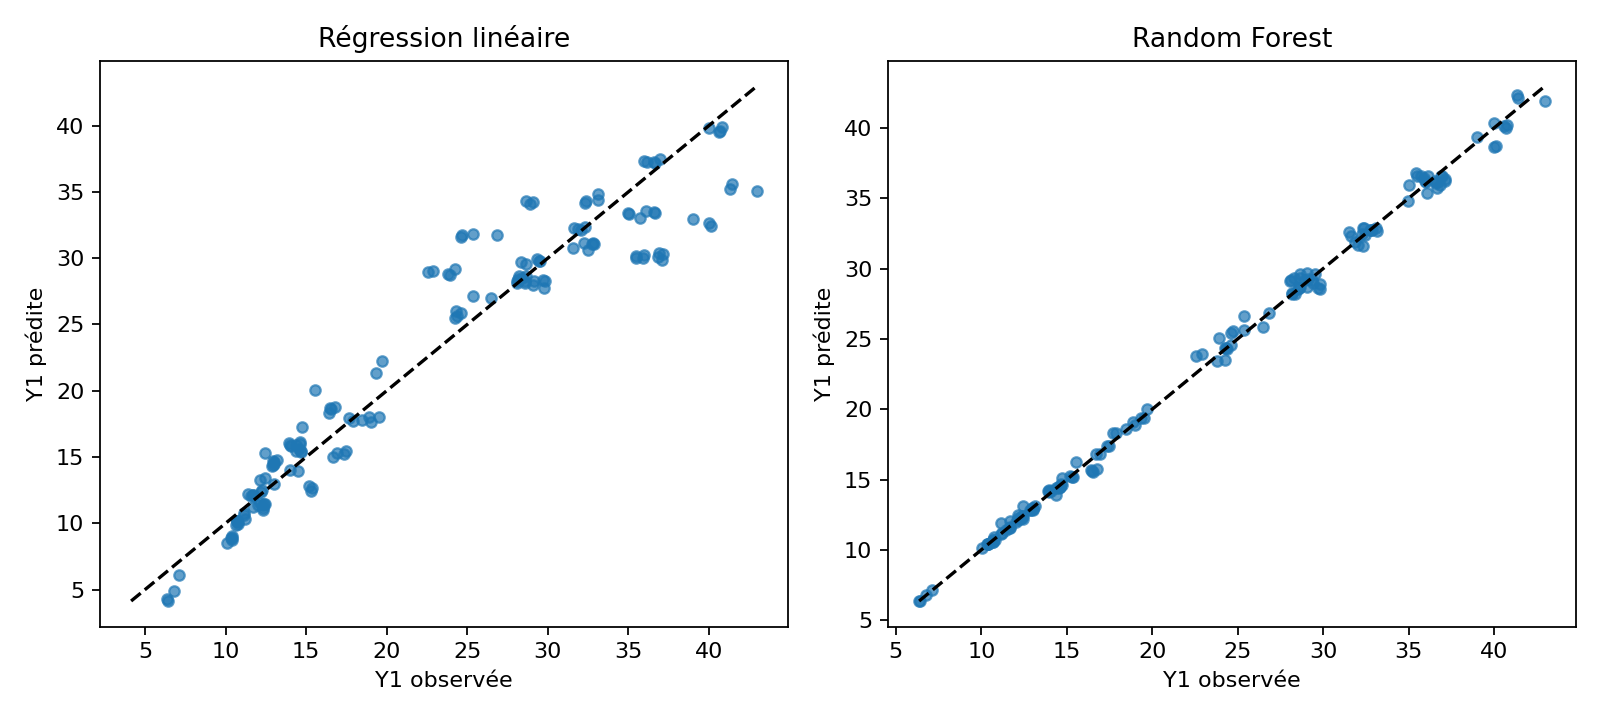
\includegraphics[width=.76\linewidth]{03_observe_predit.png}
\caption{Valeurs observées et prédites sur le test, pour la référence linéaire et Random Forest. La diagonale correspond à une prédiction parfaite.}
\end{figure}
\begin{figure}[H]\centering
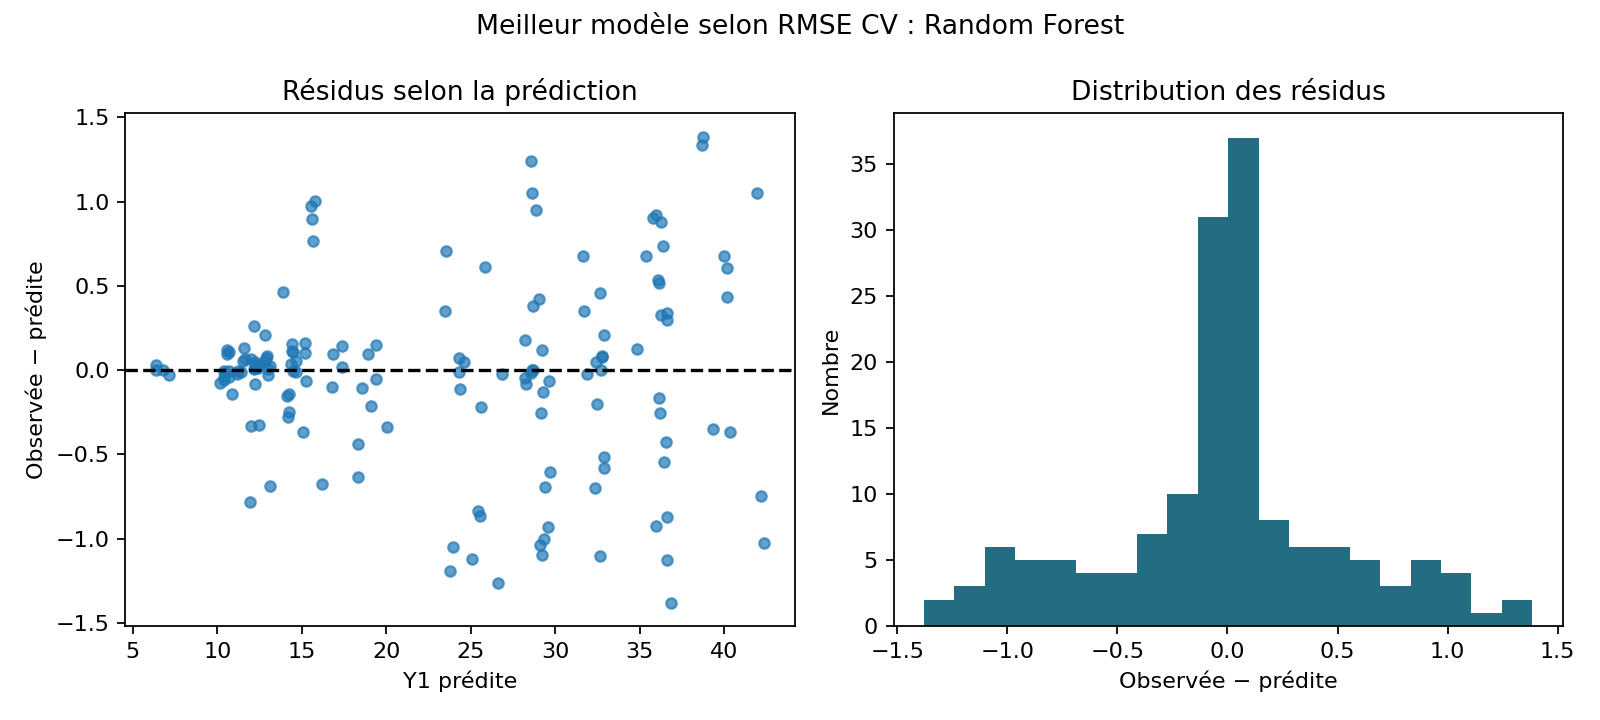
\includegraphics[width=.76\linewidth]{04_residus.png}
\caption{Résidus de Random Forest sur le test : valeur observée moins valeur prédite.}
\end{figure}
Les approches non linéaires obtiennent ici des erreurs nettement plus faibles que les modèles linéaires. Les résidus de Random Forest restent globalement proches de zéro mais comportent des écarts. Le fichier \texttt{results/erreurs\_par\_groupe.csv} décrit aussi les erreurs absolues selon la hauteur ($X_5$), l'orientation ($X_6$) et les vitrages ($X_7$, $X_8$). Par exemple, la MAE observée est de 0,171 pour $X_5=3{,}5$ (72 cas), contre 0,546 pour $X_5=7$ (82 cas). Ces écarts sont descriptifs : les sous-groupes diffèrent possiblement sur d'autres variables et leurs tailles sont limitées. Ils ne permettent donc pas d'attribuer l'erreur à la seule hauteur.

\paragraph{Limites et conclusion.} Les données représentent 768 configurations simulées et le test une seule partition de 154 cas. Les résultats ne démontrent pas une performance identique sur des bâtiments réels. Une validation externe et une étude plus complète des erreurs seraient nécessaires avant tout usage pratique. Dans le cadre de ce protocole, Random Forest est le meilleur choix selon la validation croisée ; l'arbre et la forêt ont des performances finales très proches.

\smallskip\noindent\textbf{Source des données :} UCI Machine Learning Repository, \emph{Energy Efficiency}, dataset 242. \url{https://archive.ics.uci.edu/dataset/242/energy+efficiency}.
\end{document}
